\section{Создание простого оконного приложения}
\verb|Задание.| Разработать приложение для вычисления факториала по \newline приведенному примеру.

Создано окно приложения, содержащее два элемента 
\verb|TextBox|, два элемента \verb|label| и один элемент 
\verb|Button|. Для отображения ошибок добавлен элемент \newline \verb|ErrorProvider| \cite{microsoft_provider} (см. рисунок \ref{fig:factorial_form}).
\begin{figure}[H]
    \centering
    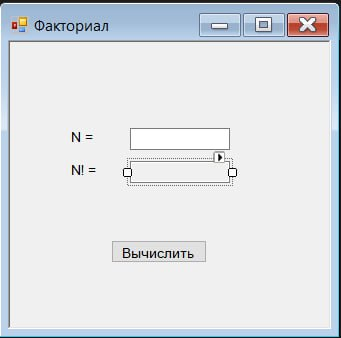
\includegraphics{../img/factorial/factorial_form.png}
    \caption{Вид формы программы вычисления факториала}
    \label{fig:factorial_form}
\end{figure}

У элементов формы изменены значения некоторых свойств \cite{microsoft_create}.
Значения измененных атрибутов представлены в таблице \ref{table:factorial_params}.

\begin{table}[H]
    \small
    \caption{Значения атрибутов элементов формы}
    \begin{tabular}{|l|l|}\hline
    Свойство & Значение\cr\hline
    \multicolumn{2}{|l|}{Форма}\cr\hline
    \verb"Text" & \verb"Факториал"\cr\hline
    \verb"FormBorderStyle" & \verb"Fixed3D"\cr\hline
    \verb"MaximizeBox" & \verb"False"\cr\hline
    \multicolumn{2}{|l|}{Первая надпись}\cr\hline
    \verb"(Name)" & \verb"label_input"\cr\hline
    \verb"Text" & \verb"N ="\cr\hline
    \multicolumn{2}{|l|}{Вторая надпись}\cr\hline
    \verb"(Name)" & \verb"label_output"\cr\hline
    \verb"Text" & \verb"N! ="\cr\hline
    \multicolumn{2}{|l|}{Первое текстовое поле}\cr\hline
    \verb"(Name)" & \verb"text_input"\cr\hline
    \multicolumn{2}{|l|}{Второе текстовое поле}\cr\hline
    \verb"(Name)" & \verb"text_output"\cr\hline
    \verb"ReadOnly" & \verb"True"\cr\hline
    \multicolumn{2}{|l|}{Кнопка}\cr\hline
    \verb"(Name)" & \verb"btn_compute"\cr\hline
    \verb"Text" & \verb"Вычислить"\cr\hline
    \multicolumn{2}{|l|}{Обработчик ошибок}\cr\hline
    \verb"(Name)" & \verb"errorProvider1"\cr\hline
    \end{tabular}
    \label{table:factorial_params}
\end{table}

Для работы программы был создан отдельный файл \verb"fact.h", содержащий   
код вычисления факториала \cite{book_excs}:
\begin{minted}[linenos, style=bw, fontsize=\small, breaklines=true]{cpp}
#pragma once
long long fact(long long n)
{
    //Если n < 0, то останавливаем с кодом -1
	if (n < 0)
		return -1;
    //Если на входе 0 или 1 - возвращаем 1
	else if (n == 0 || n == 1)
		return 1;
    //Иначе осуществляем рекурсивный вызов
	else 
		return n * fact(n - 1);
}
\end{minted}
Переменная \verb|n| "--- число, для которого вычисляется факториал.

По нажатию кнопки <<Вычислить>> происходит выполнение следующего кода:
\begin{minted}[linenos, style=bw, fontsize=\small, breaklines=true]{cpp}
private: System::Void btn_compute_Click(System::Object^ sender, System::EventArgs^ e) {
    this->text_output->Text = "";
    long long input;
    bool result = Int64::TryParse(this->text_input->Text, input);
    //Если удалось прочитать число, то вычисляем 
    //факториал.
    if (result)
    {
      long long output = fact(input);
      this->text_output->Text = System::Convert::ToString(output);
    }
    //В противном случае, с помощью ErrorProvider возвращаем ошибку.
    else
      errorProvider1->SetError(text_input, "Некорректные данные");
\end{minted}

В случае корректных входных данных, программа посчитает факториал и выведет в 
\verb|text_output| (см. рисунок \ref{fig:factorial_result}).
\begin{figure}[H]
    \centering
    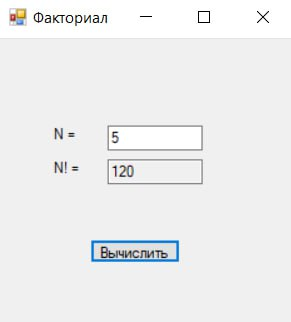
\includegraphics{../img/factorial/factoral_result.png}
    \caption{<<Факториал>>: работа программы}
    \label{fig:factorial_result}
\end{figure}

\newpage
В случае некорректных данных на входе, программа вернёт ошибку с помощью элемента 
\verb|errorProvider1| (см. рисунок \ref{fig:factorial_error}).
\begin{figure}[H]
    \centering
    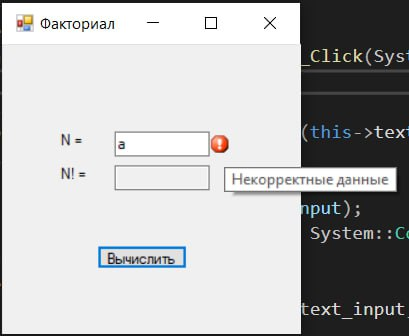
\includegraphics{../img/factorial/factorial_error.png}
    \caption{<<Факториал>>: обработка ошибок}
    \label{fig:factorial_error}
\end{figure}

С полным кодом программы можно ознакомиться в приложении \ref{app:repo}.
